
\documentclass[11pt]{article}
\usepackage[margin=0.82in]{geometry}
\usepackage{amsmath,amssymb,amsfonts}
\usepackage{booktabs,longtable,array}
\usepackage{graphicx}
\usepackage{xcolor}
\usepackage{hyperref}
\usepackage{enumitem}
\usepackage{tcolorbox}
\usepackage{microtype}
\hypersetup{colorlinks=true,linkcolor=blue,urlcolor=blue,citecolor=blue}
\title{Phase 8 Publishability Upgrade: External Validation, Benchmarks, and Gene/Pathway Sheaf Readiness}
\author{Sheaf-Theoretic Multi-Omics Brain Tumor Project}
\date{May 23, 2026}
\begin{document}
\maketitle
\begin{abstract}
This document records the next concrete upgrade toward an IEEE BIBM-quality paper. Phase 8 adds a locked internal validation audit, an external CGGA validation adapter, a gene/pathway-level regulatory sheaf scaffold, benchmark requirements, and a manuscript-safe claim plan. No external CGGA performance is claimed here because raw CGGA files were not present in the workspace.
\end{abstract}
\tableofcontents
\newpage
\section{Why Phase 8 Exists}
Phases 1--7 established a biologically constrained sheaf residual framework for glioma multi-omics. The strongest current contribution is methodological: tumor states are analyzed by residual energies induced by sheaf restriction maps, rather than by ordinary feature fusion alone. For publication, the project needs three upgrades:
\begin{enumerate}[leftmargin=*]
\item external validation, preferably TCGA-to-CGGA;
\item strict benchmark discipline against strong clinical, molecular, and graph-learning baselines;
\item higher biological resolution through gene/pathway-local residuals.
\end{enumerate}
\section{Core Method to Preserve}
Let $x_{p,v}\in \mathcal F(v)$ be patient $p$'s state at biological node $v$. For an edge $e=(u,v)$, define
\begin{equation}
 r_{p,e}=\rho_{u,e}x_{p,u}-\rho_{v,e}x_{p,v}.
\end{equation}
The global sheaf regulatory inconsistency score is
\begin{equation}
 \mathrm{SRIS}(p)=\sum_{e\in E}\|r_{p,e}\|_2^2=x_p^T L_{\mathcal F}x_p,
\end{equation}
where $L_{\mathcal F}=B_{\mathcal F}^TB_{\mathcal F}$ is the sheaf Laplacian.
\section{Phase 8 Locked Internal Audit}
A locked 25\% holdout split was used as an internal publication-readiness audit. This is not a substitute for external validation, but it helps detect overfitting and claim inflation before CGGA is added. The evaluated feature families were:
\begin{itemize}[leftmargin=*]
\item strict clinical/molecular baseline;
\item baseline plus Phase 1 SRIS and edge residuals;
\item baseline plus Phase 4 counterfactual sheaf energies;
\item baseline plus Phase 5 transport sheaf features;
\item baseline plus Phase 6 consensus discovery index;
\item baseline plus all sheaf feature families.
\end{itemize}
\begin{figure}[h]
\centering
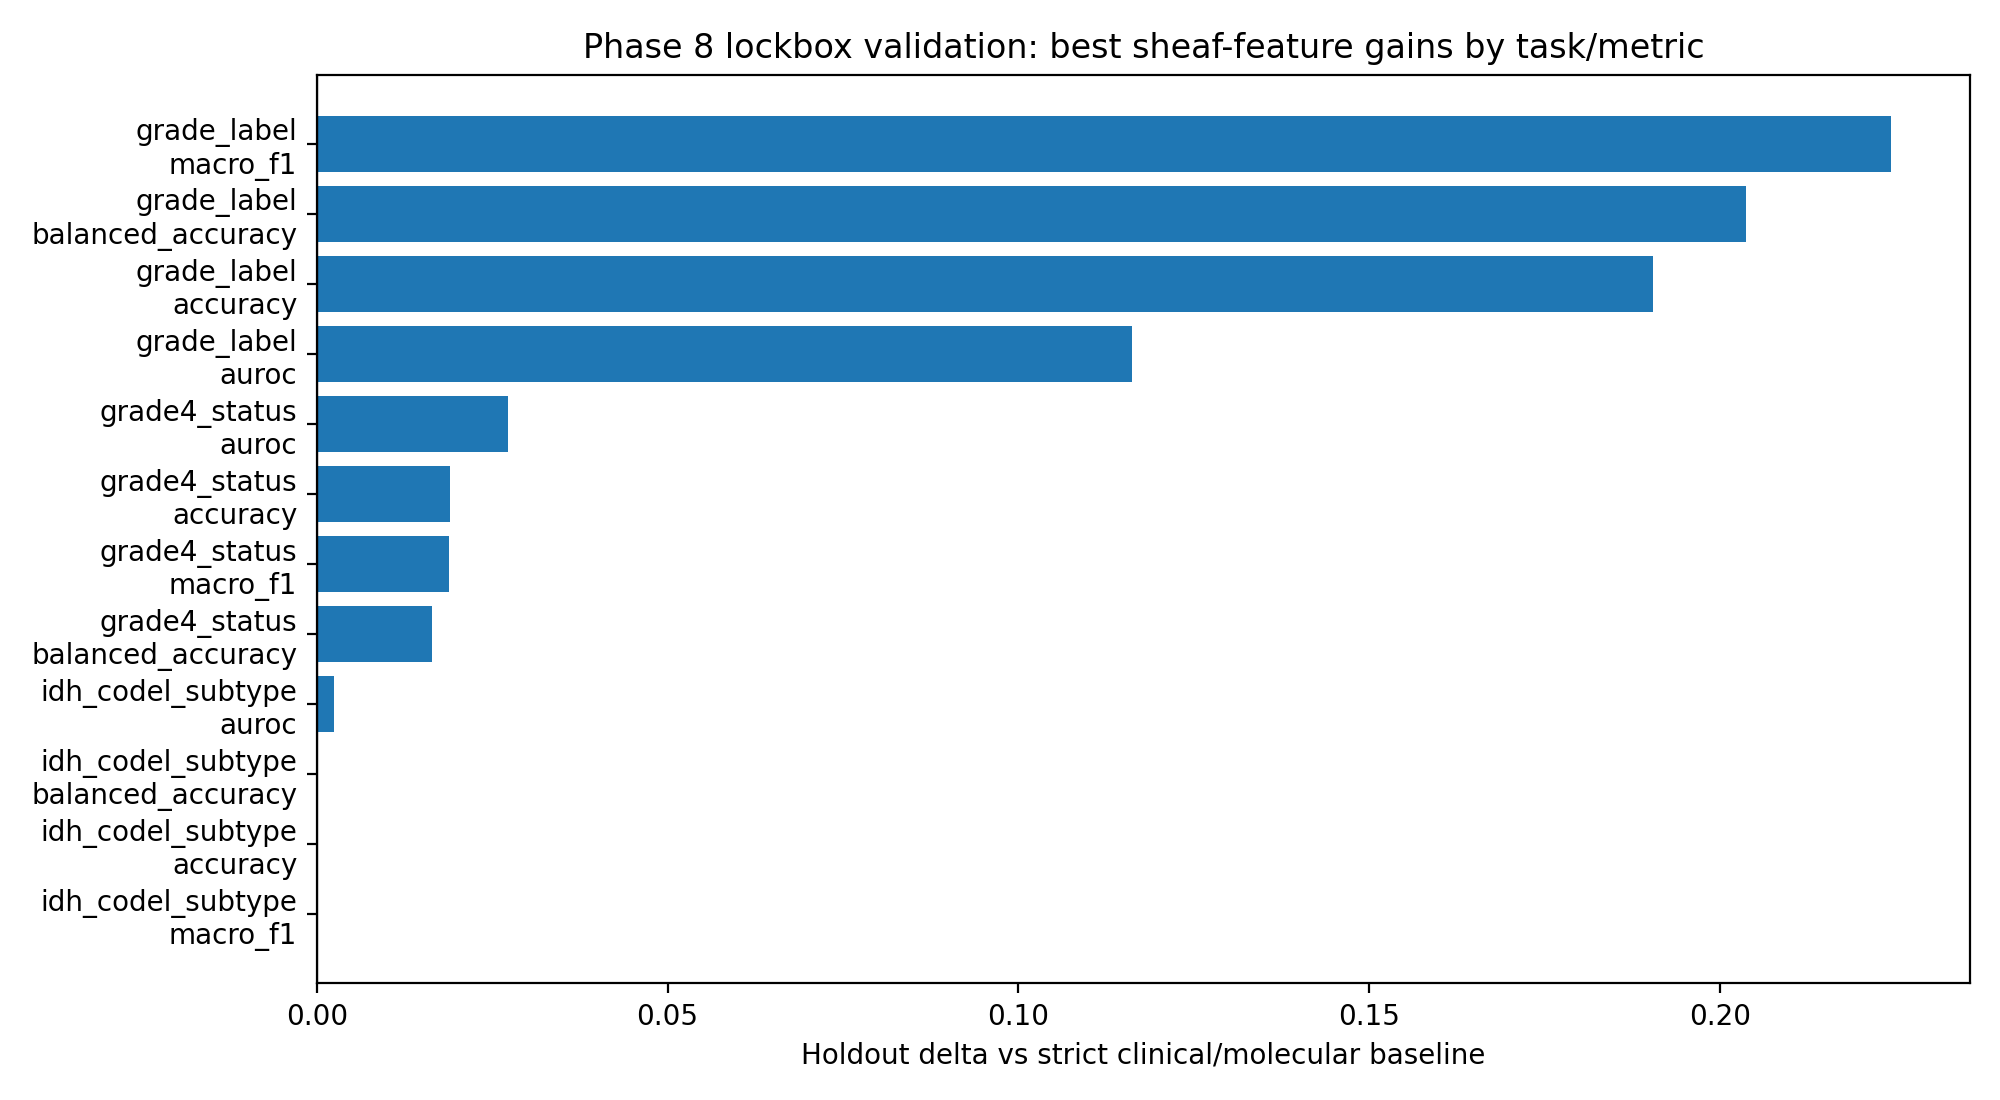
\includegraphics[width=0.95\textwidth]{../figures/phase8_best_lockbox_deltas.png}
\caption{Best locked-holdout metric deltas versus the strict baseline. Positive bars indicate that a sheaf-derived feature family improved that metric on the held-out split.}
\end{figure}
\begin{figure}[h]
\centering
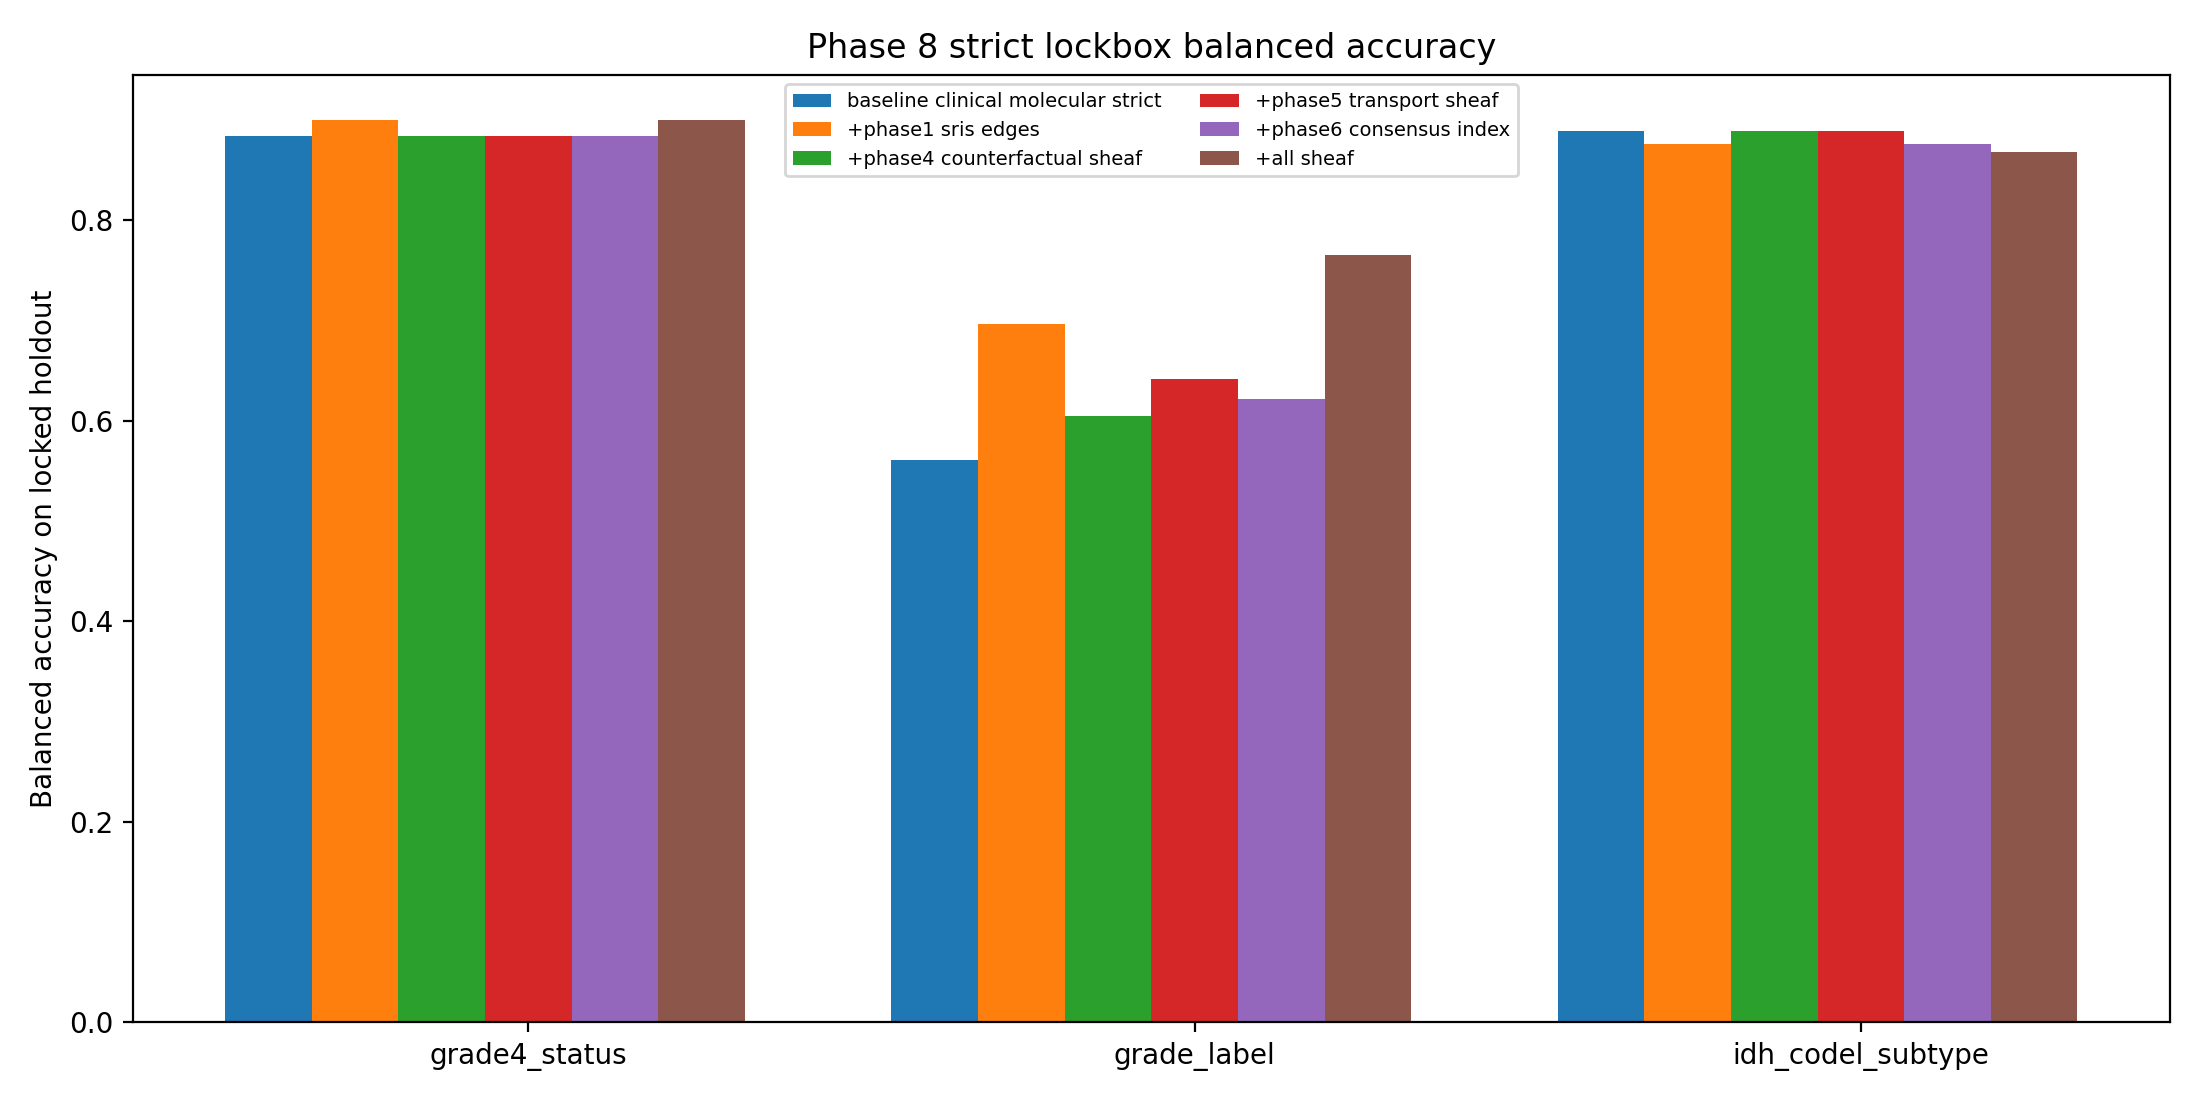
\includegraphics[width=0.95\textwidth]{../figures/phase8_lockbox_balanced_accuracy.png}
\caption{Balanced accuracy by task and feature family on the locked internal holdout.}
\end{figure}
\clearpage
\section{External Validation Protocol}
The decisive validation should train sheaf maps on TCGA and apply them to CGGA without refitting on CGGA labels. For external patient $q$, compute
\begin{equation}
 \mathrm{SRIS}_{\mathrm{CGGA}}(q)=\sum_{e\in E}\|\rho^{\mathrm{TCGA}}_{u,e}x_{q,u}-\rho^{\mathrm{TCGA}}_{v,e}x_{q,v}\|^2.
\end{equation}
Required external tests:
\begin{enumerate}[leftmargin=*]
\item external grade/subtype AUROC and balanced accuracy;
\item external survival C-index or time-dependent AUROC;
\item subgroup calibration by IDH/codel status;
\item overlap of top residual signatures across TCGA and CGGA;
\item OT stability of residual signatures across cohorts.
\end{enumerate}
\section{Gene/Pathway-Level Regulatory Sheaf}
The next major novelty upgrade is to move from summary nodes to gene/pathway nodes. For gene $g$ and patient $p$, define
\begin{equation}
 x_{p,g}=[\mathrm{RNA}_{p,g},\mathrm{Methylation}_{p,g},\mathrm{CNV}_{p,g},\mathrm{Mutation}_{p,g},\mathrm{miRNA}_{p,g}]^T.
\end{equation}
For regulatory edge $e=(u,v)$,
\begin{equation}
 r_{p,e}=\rho_{u,e}x_{p,u}-\rho_{v,e}x_{p,v}.
\end{equation}
For pathway $P$,
\begin{equation}
 \mathrm{SRIS}_{P}(p)=\sum_{e\in E(P)}\|r_{p,e}\|^2.
\end{equation}
This creates pathway-local biological discovery outputs rather than only patient-level risk scores.
\section{Benchmark Requirements}
A BIBM-quality paper should compare against:
\begin{itemize}[leftmargin=*]
\item clinical logistic/Cox baselines;
\item clinical + molecular baselines;
\item elastic-net logistic and Cox models;
\item random forest or gradient boosting;
\item graph baselines such as GCN/GAT/graph transformer if gene-level data are used;
\item identity, random, and shuffled-target sheaf controls.
\end{itemize}
\section{Manuscript-Safe Claims}
Safe current claim:
\begin{quote}
We introduce a biologically constrained sheaf residual geometry for quantifying genomic-regulatory-phenotype inconsistency in glioma multi-omics, with non-random subtype/grade geometry and strict internal validation safeguards.
\end{quote}
Unsafe until CGGA is run:
\begin{quote}
The method achieves clinical survival state of the art.
\end{quote}
\section{What Must Happen Before Submission}
\begin{enumerate}[leftmargin=*]
\item Add CGGA clinical and matched omics files.
\item Run the external adapter and TCGA-to-CGGA sheaf scoring.
\item Add pathway/gene-level residuals if matched omics are available.
\item Re-run all ablations and benchmark models on identical splits.
\item Update claim ledger using external metrics only.
\item Write final IEEE two-column manuscript from the skeleton.
\end{enumerate}
\end{document}
